\section{Preprocessing using optical flow}

\begin{comment}
\begin{frame}{Preprocessing}
    \begin{itemize}
    \item Frame size of $(640,480,3)$ pixels
    \item Cut off last 60 pixels, to remove black frame inside the car
    \item Sample down the frame to half its size, due to computational limitations
    \end{itemize}

\begin{columns}[t]
\begin{column}{.45\textwidth}
\begin{center}
\only<1->{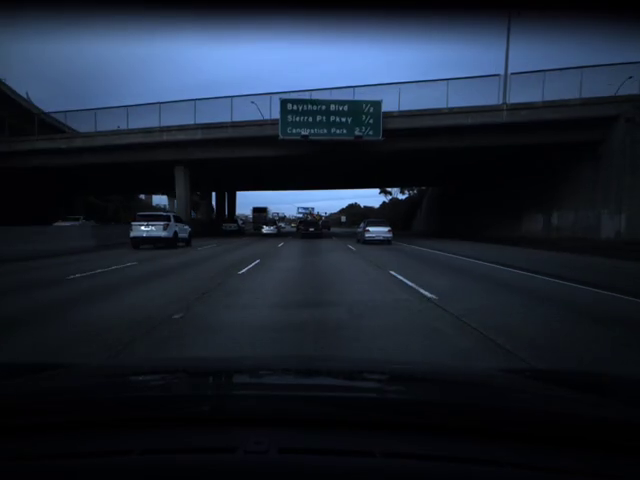
\includegraphics[width=\linewidth]{./imgs/frame2_original.png}}
\small{Original frame}
\end{center}
\end{column}
\begin{column}{.45\textwidth}
\begin{center}
\only<1->{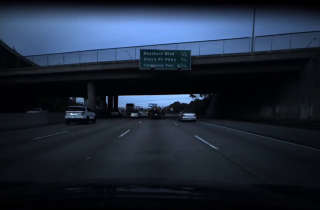
\includegraphics[width=\linewidth]{./imgs/frame2_cut_sampled.png}}
\small{Cut off the last 60 pixels, downsampled}
\end{center}
\end{column}
\end{columns}
\end{frame}
\end{comment}

\begin{frame}{Optical flow using \enquote{Farneback pyramid method}\cite{Farneback2003}}

\begin{itemize}
\item Global method to solve the optical flow equation
\begin{align*}
\partial_x f \cdot V_x + \partial_y f \cdot  V_y + \partial_t f  = 0
\end{align*}
for an image sequence $(f_t)_t$ with $f_t : \Omega \to \R^3$, for all $t$, and the (dense) flow field $V : \Omega \to \R^2, \omega \mapsto (V_x(\omega), V_y(\omega))$.
\item Uses a downsampling pyramid, to solve the equation for different resolutions of the image
\item Parameters for the Farneback method
\begin{align*}
\text{pyramid levels} &:= 3\\
\text{pyramid scaling} &:= 0.5\\
\text{window size} &:= 6\\
\text{SD of the gaussian filter} &:= 1.1
\end{align*}
\item Result: \textbf{Flow field with $(160,105,3)$ pixels}
\end{itemize}
\end{frame}

\begin{frame}{Visualization of the flow field}
\begin{itemize}
\item Flow field is a two-dimensional vector field
\item RGB representation via
\setbeamertemplate{itemize items}[circle]
\begin{itemize}
\item Transform flow field into polar coordinates $(V_x,V_y) \overset{\simeq}{\mapsto} (r, \varphi)$
\item Normalize magnitudes $r$ for the third channel
\item Values of the second channel are all set to 255
\item Multiply angle $\varphi$ by factor $\frac{180}{2\pi}$ for the first channel
\end{itemize}
\item Sample down the resolution again to speed up the training
\end{itemize}

\begin{columns}[t]
\begin{column}{.45\textwidth}
\begin{center}
\only<1->{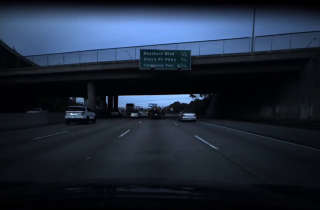
\includegraphics[width=0.85\linewidth]{./imgs/frame2_cut_sampled.png}}
\small{\\Input frame}
\end{center}
\end{column}
\begin{column}{.45\textwidth}
\begin{center}
\only<1->{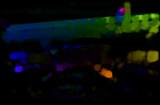
\includegraphics[width=0.85\linewidth]{./imgs/frame2_flow_field.png}}
\small{\\Corresponding flow field}
\end{center}
\end{column}
\end{columns}

\end{frame}

